\chapter{Literature Review}
\label{chapter:literature}

\section{Introduction to Scientific Workflow}
\label{sec:intro_sci_workflow}


The concept of workflow evolves from the notion of process in the manufacturing industry. These processes are the results of standardization which aims to increase efficiency by concentrating on the routine aspects of work activities. Each process represents a well-defined task, role, rule, or procedure, which is repeatedly practiced during the production of certain goods at scale. Originally all these processes are carried out by humans by manipulating physical objects. With the introduction of information technology, more and more processes can be automated with the help of computer programs. Medina-Mora et al. \cite{medina1992action} categorize processes in an organization into (a) material processes, which assemble physical components and deliver physical products; (b) information processes, which create, process, manage, and provide information, usually with the aid of computer programs; and (c) business processes, which are activities involved to fulfill a business contract or to satisfy a specific customer need. In general, multiple processes with certain orders are needed to produce a product, and some processes depend on the output of other processes. Therefore, a workflow is a logical representation of the manufacturing procedure, which includes the processes needed and the ordering of the processes, along with the dependencies between processes. As defined by the Workflow Manage Coalition \cite{hollingsworth1995workflow}, a workflow is the automation of a business process, in whole or in part, during which documents, information or tasks are passed from one participant (a resource, human or machine) to another for action, according to a set of procedural rules. This definition implies the distributed nature of workflow in that each process is executed in its own environment, while the workflow serves as the orchestration layer that glues all the processes together. 

In recent years, the concept of workflow has been applied to automate large-scale scientific computations, and assumes the term scientific workflow. Such computation usually involves a large number of different modules and services, often in the number of hundreds or thousands. The distributed nature of workflow enables the composition and execution of complex analysis on distributed resources. Examples of large-scale scientific workflows include Montage \cite{montage} \cite{web:montage}, CyberShake \cite{cybershake}, LIGO \cite{ligo}, Epigenomics \cite{bharathi2008characterization}, and SIPHT \cite{livny2008high}. Montage is an astronomical image mosaic engine, which can be used to generate custom mosaics of the sky using input images in the Flexible Image Transport System (FITS) format. CyberShake is used by the Southern California Earthquake Center (SCEC) to characterize earthquake hazards in a region using the Probabilistic Seismic Hazard Analysis (PSHA) technique. LIGO attempts to detect gravitational waves produced by various events in the universe as per Einstein`s theory of general relativity. Epigenomics is used to map the epigenetic state of human cells on a genome-wide scale by the USC Epigenome Center. SIPHT is used in bioinformatics projects at Harvard University to conduct researches for small untranslated RNAs that regulate several processes such as secretion or virulence in bacteria. Bharathi et al. \cite{bharathi2008characterization} provide a detailed review of the characteristics of the above-mentioned workflows, including their structures and computing resource consumption patterns. 

A scientific workflow consists of a set of precedence-constrained jobs can be represented by a directed acyclic graph (DAG), G = (V, E) comprising a set V = \{v\textsubscript{0}, v\textsubscript{1}, ..., v\textsubscript{n}\} of vertices and a set E = \{e\textsubscript{i,j} ..., e\textsubscript{m,n}\} of edges. As shown in Figure 1, each vertice represents a task to be executed, and each edge connects two vertices representing their precedence constraint or data dependency. In large-scale scientific workflow applications, the calculation of a workflow is usually done on a cluster with multiple computing nodes, with a scheduling algorithm to control the sequence of task execution, computing resource assignment, and data transfer. A task v\textsubscript{i} is considered as the parent task of v\textsubscript{j} if v\textsubscript{j} depends on the output of v\textsubscript{i}, and v\textsubscript{j} is considered as the child task of v\textsubscript{i}. With such a data dependency v\textsubscript{j} can not be executed until v\textsubscript{i} has completed its execution, and the output of v\textsubscript{i} has been transfer to the node where v\textsubscript{j} is to be executed. For a given workflow, the task without any parent is considered an entry task, and a task without any child task is considered an exit task. The execution time of a particular task v\textsubscript{i} is denoted as computation cost w\textsubscript{i}. The time needed to transfer data from the node running task v\textsubscript{i} to the node to run task v\textsubscript{j} is denoted as communication time c\textsubscript{i,j}. The communication time c\textsubscript{i,j} is none-zero value when tasks v\textsubscript{i} and v\textsubscript{j} are running on different nodes, but becomes zero when tasks v\textsubscript{i} and v\textsubscript{j} are running on the same node because no data transfer is needed. The time needed to execute a workflow application is defined as the makespan, or schedule length, of the workflow. 
 
\begin{figure}[!t]
	\centering
	\hspace{-5pt}
	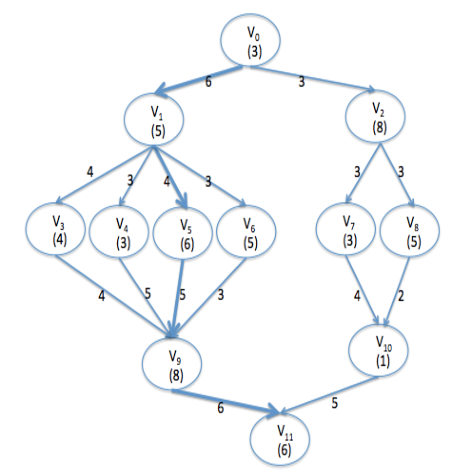
\includegraphics[width=7cm]{dag_example}
    \vspace{5pt}
	\caption{Example of a DAG representation of workflow}
	\label{fig:dag_example}
\end{figure} 

Workflow scheduling is an important aspect in workflow execution in that different scheduling algorithms might results in significant difference in makespan and resource utilization rate. The majority of these algorithms take advantage of the concept of critical path (CP), which is the longest path of the DAG representing the workflow. For a given DAG, the critical path represents the theoretical minimum time needed to finish the execution of a workflow, which is defined by the summation of the computation costs of all tasks in the critical path (which are denoted as CP-tasks). Because of its importance effect on both performance and cost, the workflow scheduling problem in general has been extensively studied and various solutions have been proposed in the literature. Representatives of such solutions include DCP (dynamic critical path), HEFT (heterogeneous earliest-finish-time), CPOP (critical path on a processor), CPF (critical path first). The majority of these studies focus either on minimizing makespan within the resource capacity available, or minimizing cost by reducing the number of nodes needed to run the workflow with a acceptable makespan. 

DCP -- Kwok et al. \cite{kwok1996dynamic} propose DCP, which assigns a task considering the critical path of partial schedule. DCP implicitly prevents the excessive (most likely unnecessary) use of processors in that for non-CP tasks it only considers processors already used in the schedule. 

HEFT / CPOP -- Topcuoglu et al. \cite{topcuoglu2002performance} present HEFT and CPOP for a bounded number of heterogeneous processors with an objective to simultaneously meet high performance and fast scheduling time. The HEFT algorithm selects the task with the highest upward rank value at each step and assigns the selected task to the processor, which minimizes its earliest finish time with an insertion-based approach. The CPOP algorithm uses the summation of upward and downward rank values for prioritizing tasks. Another difference is in the processor selection phase, which schedules the critical tasks onto the processor that minimizes the total execution time of the critical tasks. To compare HEFT and CPOP with other workflow scheduling algorithms, the authors designed a parametric graph generator to generate weighted directed acyclic graphs with various characteristics. The result shows that HEFT and CPOP can achieve shorter makespan with small cost.

PCP -- Abrishami et al. \cite{abrishami2012cost} proposed the partial critical path algorithm to minimize cost while trying to meet the user-defined deadline of a given workflow, taking advantage of the negotiable pricing mechanism of utility grids. For a given workflow, the algorithm first assigns sub-deadlines to CP tasks and to remaining tasks based on deadlines of CP tasks. Then the algorithm schedules tasks in the cheapest service that can satisfy the sub-deadline constraints. 

CPF -- Lee et al. \cite{lee2013stretch} proposed the critical path first algorithm with the assumption of resource abundance in a public cloud environment. The CPF algorithm first stretches out the schedule to proactively preserve critical path length, which is the shortest possible time of completion, then compacts the schedule for resource efficiency by rearranging tasks making use of idle/inefficiency slots present in the schedule. With this two-step approach CPF optimizes both the makespan and the resource utilization rate.

In general, the workflow scheduling problem has been studied extensively and thoroughly, with various solutions pushing both performance and cost to their limits. Unless there emerges a new form of computing resource that can be leveraged by workflow, there exists very little space for improvement in workflow scheduling.

\section{Workflow Execution Frameworks}
\label{sec:workflow_execution_frameworks}


A large-scale workflow application is usually run in a cluster with multiple nodes, with hundreds and even thousands of tasks with data and priority dependencies. The execution of a workflow involves multiple repeating steps including job scheduling, resource reservation and provisioning, data staging, job execution, status update, and fault tolerance. As scientific workflows are becoming increasingly large-scale and complex, their distributed execution across multiple resources is far beyond an average task. Due to the complexity of the workflow execution process, various workflow execution frameworks have been developed to automate this process. Some of the popular workflow execution frameworks being used in large-scale scientific computing include Condor \cite{couvares2007workflow} \cite{litzkow1988condor}, Pegasus \cite{deelman2004pegasus}, Kepler \cite{altintas2004kepler}, Taverna \cite{oinn2004taverna}, Trident \cite{barga2008trident} \cite{simmhan2009building}[21], Apache Airavata \cite{marru2011apache}, and Polyphony \cite{shams2010polyphony}. 

Condor is one of the earliest versions of workflow execution framework. Originally it was designed to harvest idle computing resource by scheduling jobs to idling UNIX workstations. With techniques such as local shadow process, job checkpointing and migration, and fair access to remote cycles, Condor was able to schedule and execute jobs utilizing idling computing resource with minimum impact on local user activities, as well as protecting the rights of light users against heavy users. Gradually Condor evolves into a feature-reach workflow execution framework, with a focus on high-throughput computations. In particular, the DAGMan module in Condor has been widely adopted by the scientific-computing community.

Pegasus stands for Planning for Execution in Grids. It is a workflow execution framework that can map complex workflows onto the Grid. Pegasus takes an abstract description of workflow in the form of a DAG, and finds the data and computing resource that are capable of executing the workflow, resulting in an executable workflow which is denoted as the concrete workflow. In the concrete workflow all jobs are bound to specific Grid resources, with necessary utilities to stage data in and out of the execution environment. Pegasus was released as part of the GriPhyN Virtual Data Toolkit, and has been used in a variety of applications ranging from astronomy, biology, gravitational-wave science, and high-energy physics.

Kepler was built upon Ptolemy II, a dataflow-oriented workflow execution framework, with some advanced extensions. In Kepler, a director module controls the execution of a workflow, while individual jobs and data transfer are implemented as reusable actors representing data source, sinks, data transformers, analytical steps, or arbitratory computational steps. Kepler provides an intuitive GUI with which scientists can easily design, prototype, execute, and analyze reusable scientific workflows. The web and grid service actor in Kepler allows scientists to utilize computation resources on the network, especially scientific computing grids. Kepler actors can be local Java threads (default), distributed execution threads via web and grid services, or libraries written in other languages invoked via Java Native Interface (JNI). Kepler acts as an agent between the computing infrastructure (such as grid, cluster, web services, data transfer) and the scientists, allowing scientists to focus on their own problem domain. 

Taverna was developed as a tool for the composition and enactment of bioinformatics workflows for the life science community. In Taverna, scientists can define their workflows in a domain-specific language called the simple conceptual unified flow language (Scufl), in which each step in the workflow represents on atomic task. Taverna provides a GUI with which scientists can composite workflows without learning the Scufl language. With the increasing number of bioinformatics databases and computational programs being made available as web services, Taverna enables researchers to take full advantages of such resources by automating the data searching and data staging processes for workflow execution. In a similar fashion, the Scufl workflows created using Taverna are resources in their own right that can be shared among scientists. 

Trident is a scientific workflow workbench built on top of Windows Workflow Foundation, a commercial workflow enactment engine designed for the Windows operating system. The Trident registry serves as a catalog of known data sets, services, workflows and activities, and compute resources, as well as maintaining state for all active workflows. Trident include a visual workflow composer in which scientists can author a workflow using the above-mentioned existing components from the service catalog. Trident also has a web portal, which allows scientist to launch and manage workflows from any location that has an Internet connection. One of the innovations in Trident is a data access layer that abstracts the actual storage service used from the workflows. So a workflow can read and/or write data objects that are transparently mapped to the target data source. Currently Trident supports a default XML store and SQL Server for local storage, and Amazon S3 and SQL Azure Data Services for Cloud storage. The fact that Trident is tightly bound to the Windows operating system makes it less appealing to scientists, which prevents its adoption in the scientific workflow community.

The Apache Airavata project was initiated to create an open development community - not just open source software - for workflow researchers. During the past researchers have created numerous toolsets and utilities for workflow research in the form of open source software. However, due to the lack of a cohesive open community, other researchers are either not aware of the availability of these tools, or are not able to evaluate the merits of these tools without extensive testing, resulting in the re-creation of similar features or functionality. The goal of the Apache Airavata project is to mitigate such continuous reinvention by fostering an open development community. The core features of the Apache Airavata project include (a) desktop and browser-based user interface; (b) server side workflow scheduling and execution framework; and (c) interoperability with third party data, workflow, and management tools. Other innovative features of the Apache Airavata project include integration with Apache Hadoop, a scalable and distributed infrastructure for big data analysis.

Polyphony is the first scientific workflow execution framework designed with the principles of cloud computing. All previous scientific workflow execution frameworks are designed with a known set of computing resources, and try to map computing tasks to available computing resources with the goal to minimize makespan. Such a design philosophy naturally lead to the master-slave architecture with stateful implementations. The workflow execution framework acts as the master assigning tasks to the computing slaves, as well as data staging and keeping tract of the status of nodes, tasks, and data. Such workflow execution frameworks favor homogeneous computing environments in which all computing nodes have similar configurations in terms of CPU, memory, and storage. Polyphony, on the contrary, takes a publisher/subscriber approach. In Polyphone, a workflow scheduling module publishes tasks to be executed to a distributed queue in the form of messages when the data dependencies are met. Multiple worker nodes can subscribe to the queue pulling tasks to be executed, and uploading the output data to the desired location based on the instructions given by the message obtained from the queue. The workflow scheduling module dynamically examines the execution progress of the whole workflow, and publishes new tasks that meet data dependencies to the queue. With such a design Polyphony does not have a central module trying to keep tract of any or all the nodes, and does not even need to have any knowledge about the configurations of the nodes. In fact, the worker nodes are not being managed in any way, and do not have any status to maintain. Any computer - Linux servers, personal laptops, cloud instances, or supercomputers - can install a software application to become and worker node and check out tasks from the distributed queue, process the task and return the output to the desired storage services, such as NFS and Amazon Simple Storage Services (S3) . In order to integrate an application into the Polyphony framework, developers will need to write a module and include it in the Polyphony distributions to be installed onto the worker nodes. 

As we can see, the majority of existing scientific workflow execution frameworks are designed with a known set of computing resources, and try to map computing tasks to available computing resources with the goal to minimize makespan. Polyphony, on the other hand, distributes tasks with a queue with the assumption that worker nodes are abundant and will automatically check out and process the tasks. These two cases represent two extreme situation in scientific computation - resource constraint in a grid environment and resource abundance in a public cloud environment. These is another situation that has not been supported by any existing workflow execution framework - a dynamical environment where the number of worker nodes is changing to address resource utilization and cost constraints in public clouds. For example, for a long running complex scientific workflow, the demand for computing resource varies at different phase of the computation. When there are a lot of parallel tasks it might be needed to spin up more worker nodes to reduce makespan. When there are only a few long running tasks it might be needed to shut down some worker nodes to reduce resource consumption. The demand for such dynamic scaling support might not seem to be very attractive with the hourly billing plan provided by AWS, but makes more sense with more fine-grained billing mechanisms such as the per-minute billing plans provided by Google Compute Engine (GCE) and Windows Azure.  

All existing scientific workflow execution frameworks focus heavily on the composition and execution of the workflow, but offers very limited capabilities in the post-processing of the workflow. The workflow scheduling and execution traces are usually written to a text file, in most cases in XML format. For a large-scale workflow with thousands of tasks, scientists can only calculate the overall resource utilization such as the total or percentage amount of time being used for computation and data staging, but the details about the scheduling and execution are often overwhelmed by the size of the output. It would be helpful for scientists - especially workflow researchers - to have a tools that can visualize the resource utilization status of all worker nodes during the whole makespan. Such a tool can provide insights into the idling time slots in the computing environment, which will help researchers design better workflow scheduling algorithms or resource allocation strategies.

\section{Workflow Execution in the Cloud}
\label{sec:workflow_execution_cloud}

In recent years, cloud computing is gaining increasing adoption in the scientific computing community. The seemingly unlimited computing resource is very attractive to researcher, who have long suffered resource deficit with the computing facilities they have access to. It is important to note that the expense of using 1000 worker nodes for 1 hour is the same as the expense of using 1 worker node for 1000 hours in a public cloud. This is a crucial benefit to any application; expediency of computational result comes for free simply due to the elasticity available in the cloud.

Early studies on doing scientific workflows on public clouds tried to determine the benefits and drawbacks of cloud computing for scientific applications, with a focus on performance and cost. Juve et al. \cite{juve2009scientific} examine the performance of doing scientific workflow in Amazon EC2 using three characteristic workflows - Montage, Broadband, and Epigenome - and compare the result with a typical HPC system built with the NCSA`s Abe cluster. The results indicate the primary advantage of Abe is the availability of a high-speed interconnect, as well as a parallel file system that significantly improve the performance of I/O-intensive applications. In fact, the performance of EC2 instances is very close to that of Abe when  the Abe cluster is using the local disks for storage. The primary cost of doing scientific workflows on public clouds lies in acquiring resources to execute workflow tasks. The storage cost is relatively small, and data transfer cost can be reduced by storing data in the cloud rather than transferring it for each workflow.

Juve et al. \cite{juve2010data} \cite{juve2012evaluation} further investigate the I/O problem associated with doing scientific worflows on public clouds, exploring various data sharing options on Amazon EC2. In grids and HPC clusters, workflow data is often stored on network and parallel file systems, which are not available in public clouds. The authors investigate ways to store and share data for scientific workflows in the cloud, including Amazon S3, NFS, GlusterFS, and PVFS. Experiments are carried out with three characteristic workflows - Montage, Broadband, and Epigenome. The results indicate that GlusterFS delivers good performance for all the applications tested and seems to perform well with both a large number of small files. NFS performs well when the number of clients is small or the workload is not I/O-intensive. Both PVFS and S3 perform poorly on workloads with a large number of small files. In general, the storage systems that produce the best workflow runtimes result in the lowest cost.

Deelman et al. \cite{deelman2008cost} study the cost of running scientific workflows on the cloud with various compute, storage, and communication options. Using the Montage application and Amazon EC2 as a case study, the authors determine that for a data intensive application with a small computational granularity, the storage costs is insignificant as compared to the computation cost. Other researchers, such as Juve et al. \cite{juve2009scientific} \cite{juve2010data} \cite{juve2012evaluation}, also agree that cloud computing offers a cost-effective solution for scientific workflow applications.

Computing resources on public clouds, as well as scientific grids, should be considered as fragile where faults are likely to occur. In Amazon EC2, a user`s VM instances might be terminated because of a fault on the underlying server hardware. Without sophisticated fault handling, workflows are frequently abandoned when a fault occurs, leading to a waste of computing resource. Ramakrishnan et al. \cite{ramakrishnan2009vgrads} study the execution of time-sensitive scientific workflows on the cloud with special considerations on fault tolerance. Probabilities of tasks completing are computed using the failure probability of the computing resource and the failure probabilities of its parent tasks. To increase the probability of success for each workflow task, the workflow planner interacts with a fault tolerance component to determine if a task should implement replication. Juhnke et al. \cite{juhnke2009fault} propose a fault tolerance module to be used with ActiveBPEL, an open source workflow enactment engine, to handle infrastructure faults for long-running workflows. By pre-classifying the possible faults in the infrastructure, policies are configured to invoke automatic recovery by providing redundancy resources using public clouds such as Amazon EC2. As compared to \cite{ramakrishnan2009vgrads} and \cite{juhnke2009fault}, which involves complicated techniques in determining the status of both the infrastructure and the tasks, the Polyphony workflow execution framework \cite{shams2010polyphony} offers a much more elegant solution to the fault tolerance problem using characteristics of the Amazon Simple Queue Service (SQS). In Polyphony, tasks are published to a distributed queue, while worker nodes actively pull the queue to check out tasks for processing. Once a task has been checked out by a worker node, it becomes invisible to other worker nodes within a certain timeout period. When the worker node finish processing the task, it uploads the output to the desired storage service, and deletes the task from the queue. If the task has not been deleted from the queue after the timeout period, which is an indicator that the task has not been successfully processed, it becomes visible to all worker nodes again, and can be checked out and processed by other worker nodes. With such a mechanism any worker nodes can fail at any time without affecting the successful execution of the workflow.

Traditionally, workflow scheduling focuses on the minimization of makespan with tightly coupled computer systems like clusters. When moving to the public cloud environment, scientists usually pre-allocate a certain number of VM instances so that they can execute workflows in a way similar to traditional clusters. Because of the data dependencies and priorities of the tasks, it is inevitable that some worker nodes might be idling for a considerably long period of time during the execution. This represents further cost optimization opportunities in that scientists can terminate instances that are waiting for tasks to be available, and launch instances when additional computing resource is needed. Dornemann et al. \cite{dornemann2009demand} present an on-demand resource provisioning solution for BPEL workflows using Amazon EC2. Experiments are carried out with the ActiveBPEL workflow enactment engine and computational intensive video analysis applications to verify the visibility of the solution. Ostermann et al. \cite{ostermann2010dynamic} study some specific techniques for dynamically provisioning computing resource on Amazon EC2 for scientific workflows, including cloud start, instance type, grid scheduling, and cloud stop. Nagavaram et al. \cite{nagavaram2011cloud} presented a case study using a dynamic workflow for mass spectrometry data analysis on Amazon EC2. In order to effectively use cloud resources, researchers parallelize the search method in MassMatrix, an application which searches proteins and peptides from tandem mass spectrometry data. A flexible workflow was created with the Pegasus to guide the data analysis process. Finally, a dynamic resource allocation module (an extension of Pegasus/Wrangler) was created to launch or terminate VM instances based on a time constraint specified by the user. Experiments with several different datasets indicate that this technique scales quite well, and is effective in meeting time constraints. One other aspect, although not explicitly emphasized by the authors, is that rewriting some critical components of the tasks (such as the search method in MassMatrix) is needed to take full advantage of public clouds. 


\section{Research Directions}
\label{sec:research_directions}


This literature review makes the following observations regarding researches on scientific workflows:

Workflow scheduling algorithms have been studied extensively, with only very limited space in workspan optimization.  This is particularly true with a traditional computer cluster where the total amount of computing resource is pre-allocated and does not change over the makespan. However, in a public cloud environment where computing resource is abundant, there exist opportunities for cost optimization with dynamic resource allocation and termination. There have been some research efforts exploiting dynamic resource allocation on Amazon EC2, which offers an bill-by-hour mechanism. New public clouds - such as Google Compute Engine and Windows Azure - are offering bill-by-minute mechanism. Such a finer grained billing mechanism represents further cost optimization opportunities, and deserves the attention from the scientific workflow research community.

In the past, resource scarcity was a great challenge for the scientific computing community. Most researchers depend on grid computing to obtain access to large scale computing resource. In a grid environment, researcher are confronted with resource heterogeneity in compute, networking, and storage. In recent years, public clouds are gradually making their way into the scientific computing community and gaining increasing level of adoption. As compared to a grid environment, a public cloud offers seemingly unlimited amount of computing resource where a large scale homogeneous computing environment can be constructed on demand. Despite the significant difference between the grid environment and the public cloud environment, many researchers in the scientific workflow community continue to use methodologies and tools developed for grid computing in public clouds. This results in significant resource under utilization as well as over spending. 

In order to utilize public clouds in a more cost-effective way, further research is needed in the following directions:

(1) How do we optimize the execution of scientific workflows in public clouds?

(2) Can we use existing tools and methodologies directly in public clouds, or new tools and methodologies are needed for public clouds?

(3) How do we optimize the execution of large-scale scientific workflow ensembles in public clouds to meet both cost and deadline constrains?



